% =====================================================================
%  CONTOH TERISI -- PROPOSAL SKRIPSI (data fiktif untuk memperagakan format)
%  S1 Rekayasa Sistem Komputer, Fakultas Teknik, UM Buton
%  Kompilasi PDF : xelatex (lihat menu.sh)   |   Word : pandoc (lihat menu.sh)
%  Ukuran dan tata letak sama dengan Seminar Hasil dan Skripsi: A4; margin kiri/atas/kanan/bawah
%  = 4/4/3/3 cm; Times New Roman 12 pt; 1,5 spasi; judul "BAB I" di tengah, tiap bab mulai halaman baru.
%  Isi dipisah per bab di folder bab/ ; ubah isi di sana.
% =====================================================================
\documentclass[12pt,a4paper]{report}
\usepackage{skripsi}
\usepackage{skripsi-bab}

% ---------- Data dosen & peran (common/dosen.tex, common/peran.tex) ----------
% =====================================================================
%  DAFTAR DOSEN  --  Program Studi Rekayasa Sistem Komputer, UM Buton
%  Satu dosen = dua makro:  \dsnKunci (nama dan gelar)  dan  \nidnKunci (NIDN).
%  Tambah dosen baru dengan menyalin dua baris di bawah. Peran (pembimbing, penguji, dst.)
%  diatur di peran.tex atau lewat  ./menu.sh  ->  "Atur dosen / peran".
% =====================================================================
\newcommand{\dsnAwaluddin}{Muhammad Awaluddin, S.Kom., M.Kom}
\newcommand{\nidnAwaluddin}{0909038201}
\newcommand{\dsnDarmawan}{Darmawan, S.Kom., M.Kom}
\newcommand{\nidnDarmawan}{0911048204}
\newcommand{\dsnRando}{Rando, S.Kom., M.Eng.}
\newcommand{\nidnRando}{0911069501}
\newcommand{\dsnSaidi}{La Ode Muhammad Saidi, S.Si., M.Kom}
\newcommand{\nidnSaidi}{0913038905}
\newcommand{\dsnDidin}{Didin Adri, S.Si., M.Sc}
\newcommand{\nidnDidin}{0930088802}
\newcommand{\dsnHibrian}{Muhammad Hibrian Wiwi, S.T., M.Kom}
\newcommand{\nidnHibrian}{0930129003}
\newcommand{\dsnRasyid}{Muhammad Abdur Rasyid Asruddin, S.T., M.Kom}
\newcommand{\nidnRasyid}{6641774675130242}
% Dekan Fakultas Teknik
\newcommand{\dsnAgusman}{Agusman, S.T., M.M}
\newcommand{\nidnAgusman}{0917088206}

% =====================================================================
%  PERAN DOSEN  --  dipakai otomatis di sampul, lembar persetujuan/pengesahan,
%  kata pengantar, dan abstrak semua dokumen.
%  Isi dengan kunci dosen dari dosen.tex, mis.  \dsnAwaluddin  dan  \nidnAwaluddin.
%  Atau jalankan  ./menu.sh  lalu pilih "Atur dosen / peran"  (berkas ini ditulis ulang otomatis).
% =====================================================================
\newcommand{\PembimbingI}{…………………}\newcommand{\PembimbingInidn}{……………………}
\newcommand{\PembimbingII}{…………………}\newcommand{\PembimbingIInidn}{……………………}
\newcommand{\PengujiI}{…………………}\newcommand{\PengujiInidn}{……………………}
\newcommand{\PengujiII}{…………………}\newcommand{\PengujiIInidn}{……………………}
\newcommand{\KetuaProdi}{…………………}\newcommand{\KetuaProdinidn}{……………………}
\newcommand{\Dekan}{\dsnAgusman}\newcommand{\Dekannidn}{\nidnAgusman}

% Peran dosen pada CONTOH ini hanya ilustrasi (tidak mengubah common/peran.tex)
\renewcommand{\PembimbingI}{\dsnAwaluddin}\renewcommand{\PembimbingInidn}{\nidnAwaluddin}
\renewcommand{\PembimbingII}{\dsnDarmawan}\renewcommand{\PembimbingIInidn}{\nidnDarmawan}
\renewcommand{\PengujiI}{\dsnRando}\renewcommand{\PengujiInidn}{\nidnRando}
\renewcommand{\PengujiII}{\dsnSaidi}\renewcommand{\PengujiIInidn}{\nidnSaidi}
\providecommand{\satubaris}[1]{\mbox{#1}}   % cadangan (konversi Word); versi PDF ada di skripsi.sty

% ---------- Makro yang ikut dibaca pandoc ----------
\newcommand{\logo}[1]{
\includegraphics[width=#1]{../../gambar/logo-umbuton.png}}
\newcommand{\babtp}[1]{\chapter*{#1}\addcontentsline{toc}{chapter}{#1}}
\definecolor{gantt}{HTML}{FF9900}
\newcommand{\isi}{\cellcolor{gantt}\textbf{~}}   % sel terisi pada jadwal

\begin{document}

% Tambah bab baru: buat berkas bab/NN-nama.tex lalu \input di sini.
% Sampul dan lembar persetujuan pembimbing
% ============================ SAMPUL ============================
\thispagestyle{empty}
\begin{ruang}{0.4}\end{ruang}
\begin{sampulbesar}
\textbf{PROPOSAL SKRIPSI}
\end{sampulbesar}
\begin{ruang}{0.5}\end{ruang}
\begin{sampulbesar}
\textbf{ANALISIS KINERJA ALGORITMA PENJADWALAN PAKET PADA JARINGAN LTE MENGGUNAKAN SIMULATOR NS-3}
\end{sampulbesar}
% ruang kosong setinggi baris "Diajukan untuk memenuhi ..." pada sampul Skripsi, agar posisi semua sampul sama
\begin{ruang}{1.87}\end{ruang}
\begin{ruang}{0.6}\end{ruang}
\begin{tengah}
\logo{4.5cm}
\end{tengah}
\begin{ruang}{0.6}\end{ruang}
\begin{sampulsedang}
\textbf{Disusun oleh:}

\textbf{LA ODE CONTOH PRATAMA}

\textbf{NPM 2201010001}
\end{sampulsedang}
\begin{ruang}{0.8}\end{ruang}
\begin{sampulsedang}
\textbf{PROGRAM STUDI REKAYASA SISTEM KOMPUTER}

\textbf{FAKULTAS TEKNIK}

\textbf{UNIVERSITAS MUHAMMADIYAH BUTON}

\textbf{BAUBAU}

\textbf{2026}
\end{sampulsedang}
\begin{halamanbaru}\end{halamanbaru}

% ============================ LEMBAR PERSETUJUAN ============================
\thispagestyle{empty}
\begin{tengah}
\textbf{\underline{PROPOSAL SKRIPSI}}
\end{tengah}

\begin{tanpagaris}
\begin{longtable}{@{}p{0.16\linewidth}p{0.04\linewidth}p{0.74\linewidth}@{}}
Nama & : & La Ode Contoh Pratama \\[6pt]
NPM & : & 2201010001 \\[6pt]
\textit{Contact} & : & Jl. Contoh No. 1, Baubau \\[6pt]
 & & 0812-0000-0000; contoh@example.ac.id \\
 & & {\footnotesize (alamat, telepon, email untuk kemudahan menghubungi; dan jika ada perubahan data harap segera menghubungi Program Studi)} \\
\end{longtable}
\end{tanpagaris}

\begin{ruang}{1.5}\end{ruang}
\begin{tengah}
\textbf{PERSETUJUAN PEMBIMBING}

Proposal Skripsi ini telah disetujui oleh:
\end{tengah}

\begin{tanpagaris}\begin{tabelpusat}
\begin{longtable}{@{}>{\centering\arraybackslash}p{0.48\linewidth}>{\centering\arraybackslash}p{0.48\linewidth}@{}}
\textbf{Pembimbing I}\newline ~\newline ~\newline ~\newline ~\newline ~\newline ~\newline ~\newline \satubaris{\PembimbingI}\newline NIDN. \PembimbingInidn &
\textbf{Pembimbing II}\newline ~\newline ~\newline ~\newline ~\newline ~\newline ~\newline ~\newline \satubaris{\PembimbingII}\newline NIDN. \PembimbingIInidn \\
\end{longtable}
\end{tabelpusat}\end{tanpagaris}
\begin{akhirsampul}\end{akhirsampul}
      % sampul, lembar persetujuan (tanpa nomor halaman)
% Abstrak (Indonesia dan Inggris)
\babtp{ABSTRAK}
\begin{abstrak}
Jaringan Long Term Evolution (LTE) membagi sumber daya radio kepada pengguna melalui penjadwal paket, sehingga pemilihan algoritma penjadwalan memengaruhi throughput dan keadilan layanan. Penelitian ini bertujuan mengukur throughput total dan indeks fairness Jain pada algoritma Round Robin (RR), Proportional Fair (PF), dan Max C/I, serta menentukan algoritma dengan kompromi terbaik. Penelitian dilaksanakan dengan simulator ns-3 pada satu sel LTE berlebar pita 20 MHz dan jumlah pengguna 10 sampai 50 yang bergerak acak. Setiap skenario diulang sebanyak 10 kali dengan seed berbeda dan hasilnya dirata-ratakan. Hasil yang diharapkan adalah gambaran kuantitatif kinerja ketiga algoritma, dengan dugaan bahwa Max C/I memberikan throughput tertinggi, RR keadilan tertinggi, dan PF kompromi terbaik. Penelitian ini diharapkan menjadi bahan pertimbangan dalam memilih algoritma penjadwalan pada perancangan jaringan LTE.

\textbf{Kata kunci:} throughput, fairness, penjadwalan paket, LTE, ns-3.
\end{abstrak}

\begin{halamanbaru}\end{halamanbaru}
\babtp{ABSTRACT}
\begin{abstrak}
The Long Term Evolution (LTE) network allocates radio resources to users through a packet scheduler, so the choice of scheduling algorithm affects throughput and service fairness. This research aims to measure the total throughput and Jain's fairness index of the Round Robin (RR), Proportional Fair (PF), and Max C/I algorithms, and to determine the algorithm with the best compromise. The research will be carried out using the ns-3 simulator on a single LTE cell with a 20 MHz bandwidth and 10 to 50 randomly moving users. Each scenario will be repeated 10 times with different seeds and the results averaged. The expected result is a quantitative picture of the performance of the three algorithms, with the hypothesis that Max C/I provides the highest throughput, RR the highest fairness, and PF the best compromise. This research is expected to inform the choice of scheduling algorithm in LTE network design.

\textbf{Keywords:} throughput, fairness, packet scheduling, LTE, ns-3.
\end{abstrak}

\begin{halamanbaru}\end{halamanbaru}
     % abstrak (angka romawi)
% Daftar isi, daftar tabel, daftar gambar; setelah ini nomor halaman mulai dari 1 (isi)
\begin{daftarisi}\end{daftarisi}
\begin{daftartabel}\end{daftartabel}
\begin{daftargambar}\end{daftargambar}
\begin{akhirdepan}\end{akhirdepan}
\pagestyle{isi}

  % daftar isi; setelah ini nomor halaman mulai dari 1

% Bab I  Pendahuluan
\chapter{PENDAHULUAN}

\section{Latar Belakang}
Perkembangan layanan data seluler, seperti video bergerak, konferensi daring, dan komputasi awan, mendorong peningkatan kebutuhan kapasitas dan mutu layanan jaringan akses radio. Jaringan \textit{Long Term Evolution} (LTE) menjadi salah satu teknologi yang banyak digunakan karena menyediakan laju data tinggi dan latensi rendah (Ghosh et al., 2010; Dahlman et al., 2011).

Pada jaringan LTE, sumber daya radio pada sisi \textit{downlink} dibagi menjadi satuan \textit{resource block} (RB) yang dialokasikan kepada pengguna oleh penjadwal paket di eNodeB pada setiap interval transmisi 1 milidetik (Dahlman et al., 2011). Pemilihan algoritma penjadwalan menentukan bagaimana RB dibagikan sehingga berpengaruh langsung terhadap \textit{throughput} dan keadilan layanan antarpengguna (Capozzi et al., 2013).

Berbagai algoritma penjadwalan telah diusulkan, antara lain \textit{Round Robin} (RR), \textit{Proportional Fair} (PF), dan \textit{Maximum Carrier-to-Interference} (Max C/I). Kajian pustaka dan perbandingan skema penjadwalan menunjukkan bahwa setiap algoritma memiliki karakteristik yang berbeda (Andrews, 2007; AlQahtani \& Alhassany, 2013), dan kebutuhan penjadwalan juga berbeda pada penerapan tertentu, misalnya jaringan listrik cerdas yang menuntut penjadwalan waktu nyata (Xu \& Fischione, 2012).

Meskipun demikian, kinerja setiap algoritma sangat bergantung pada skenario, khususnya jumlah pengguna dan kondisi kanal. Oleh karena itu diperlukan kajian kuantitatif yang membandingkan ketiga algoritma pada skenario yang sama dan terkendali. Simulator jaringan ns-3 menyediakan modul LTE beserta ketiga penjadwal tersebut sehingga memungkinkan perbandingan yang dapat diulang (ns-3 Consortium, t.t.). Penelitian ini membandingkan kinerja RR, PF, dan Max C/I pada jaringan LTE dengan jumlah pengguna 10 sampai 50 menggunakan simulator ns-3.

\section{Rumusan Masalah}
Berdasarkan latar belakang tersebut, rumusan masalah penelitian ini adalah:
\begin{enumerate}
\item Bagaimana \textit{throughput} total jaringan LTE pada algoritma penjadwalan RR, PF, dan Max C/I dengan jumlah pengguna 10 sampai 50?
\item Bagaimana tingkat keadilan (\textit{fairness}) antarpengguna pada ketiga algoritma tersebut?
\item Algoritma penjadwalan manakah yang memberikan kompromi terbaik antara \textit{throughput} dan \textit{fairness}?
\end{enumerate}

\section{Tujuan Penelitian}
Tujuan penelitian ini adalah:
\begin{enumerate}
\item mengukur \textit{throughput} total jaringan LTE pada algoritma RR, PF, dan Max C/I;
\item mengukur indeks \textit{fairness} Jain antarpengguna pada ketiga algoritma;
\item menentukan algoritma dengan kompromi terbaik antara \textit{throughput} dan \textit{fairness}.
\end{enumerate}

\section{Manfaat Penelitian}
Manfaat teoretis penelitian ini adalah menambah bukti kuantitatif tentang karakteristik algoritma penjadwalan paket LTE pada variasi jumlah pengguna. Manfaat praktisnya adalah menjadi bahan pertimbangan bagi perancang dan operator jaringan dalam memilih algoritma penjadwalan, serta menjadi rujukan bagi mahasiswa yang mempelajari simulasi jaringan seluler.

\section{Batasan Masalah}
Penelitian ini dibatasi pada:
\begin{enumerate}
\item satu sel (satu eNodeB) dengan lebar pita \textit{downlink} 20 MHz;
\item trafik \textit{downlink} berupa aliran UDP dengan laju konstan;
\item tiga algoritma penjadwalan, yaitu RR, PF, dan Max C/I;
\item evaluasi melalui simulasi pada ns-3, tanpa pengujian pada perangkat nyata.
\end{enumerate}

\section{Sistematika Penulisan}
Proposal ini terdiri atas tiga bab. Bab I berisi pendahuluan. Bab II berisi tinjauan pustaka. Bab III berisi metode penelitian beserta jadwal pelaksanaan.

Seluruh angka, nama pengguna, dan alamat pada contoh ini fiktif dan hanya dibuat untuk memperagakan format penulisan.

% Bab II  Tinjauan Pustaka
\chapter{TINJAUAN PUSTAKA}

\section{Penelitian Terdahulu}
AlQahtani dan Alhassany (2013) membandingkan beberapa skema penjadwalan pada jaringan LTE untuk melihat pengaruh pemilihan skema terhadap kinerja jaringan. Capozzi et al. (2013) menyusun survei mengenai isu rancangan utama penjadwalan paket \textit{downlink} pada jaringan seluler LTE, termasuk kriteria kinerja yang menjadi dasar perbandingan algoritma. Xu dan Fischione (2012) mengkaji penjadwalan waktu nyata pada LTE untuk jaringan listrik cerdas, yang menunjukkan bahwa kebutuhan aplikasi memengaruhi pilihan penjadwal. Andrews (2007) menyajikan tinjauan teori penjadwalan pada jaringan data nirkabel yang menjadi landasan banyak algoritma penjadwalan saat ini.

\needspace{9cm}
Ringkasan penelitian terdahulu dan perbedaannya dengan penelitian ini disajikan pada Tabel 2.1.

\begin{singlespace}
\begin{longtable}{|p{0.22\linewidth}|p{0.34\linewidth}|p{0.32\linewidth}|}
\caption{Perbandingan penelitian terdahulu dengan penelitian ini}\\
\hline
\textbf{Peneliti (tahun)} & \textbf{Fokus penelitian} & \textbf{Perbedaan dengan penelitian ini} \\
\hline
AlQahtani dan Alhassany (2013) & Perbandingan beberapa skema penjadwalan LTE & Penelitian ini membandingkan RR, PF, dan Max C/I secara kuantitatif pada variasi 10--50 pengguna di ns-3 \\
\hline
Capozzi et al. (2013) & Survei isu rancangan penjadwalan paket \textit{downlink} LTE & Penelitian ini bersifat eksperimen simulasi, bukan survei \\
\hline
Xu dan Fischione (2012) & Penjadwalan waktu nyata LTE untuk jaringan listrik cerdas & Penelitian ini memakai trafik data umum, bukan trafik jaringan listrik cerdas \\
\hline
Andrews (2007) & Tinjauan teori penjadwalan jaringan data nirkabel & Penelitian ini menerapkan teori tersebut pada skenario LTE tertentu \\
\hline
\end{longtable}
\end{singlespace}

\section{Landasan Teori}

\subsection{Jaringan LTE dan Penjadwalan Paket}
LTE menggunakan \textit{Orthogonal Frequency Division Multiple Access} (OFDMA) pada sisi \textit{downlink}. Sumber daya radio dibagi dalam domain waktu dan frekuensi menjadi RB; pada lebar pita 20 MHz tersedia 100 RB yang dapat dialokasikan setiap interval transmisi 1 milidetik (Ghosh et al., 2010; Dahlman et al., 2011). Penjadwal paket di eNodeB memutuskan RB mana yang diberikan kepada pengguna tertentu berdasarkan umpan balik kualitas kanal (CQI) yang dilaporkan pengguna (Dahlman et al., 2011).

\subsection{Algoritma Penjadwalan}
Algoritma \textit{Round Robin} mengalokasikan sumber daya secara bergiliran kepada setiap pengguna tanpa memperhatikan kondisi kanal, sehingga sederhana dan adil dalam jatah waktu. Algoritma Max C/I selalu memilih pengguna dengan kondisi kanal terbaik pada setiap interval sehingga memaksimalkan \textit{throughput} sistem, tetapi pengguna dengan kanal buruk dapat jarang terlayani. Algoritma \textit{Proportional Fair} memilih pengguna dengan metrik prioritas

\begin{tanpagaris}
\begin{longtable}{@{}p{0.08\linewidth}p{0.76\linewidth}r@{}}
 & $m_{i}(t)=\dfrac{r_{i}(t)}{R_{i}(t)}$ & (2.1) \\
\end{longtable}
\end{tanpagaris}

dengan nilai:

\begin{tanpagaris}
\begin{longtable}{@{}p{0.15\linewidth}p{0.05\linewidth}p{0.7\linewidth}@{}}
$m_{i}(t)$ & = & metrik prioritas pengguna ke-$i$ pada waktu $t$ \\
$r_{i}(t)$ & = & laju data sesaat yang dapat dicapai pengguna ke-$i$ \\
$R_{i}(t)$ & = & rata-rata \textit{throughput} pengguna ke-$i$ \\
\end{longtable}
\end{tanpagaris}

Rata-rata \textit{throughput} diperbarui secara eksponensial pada setiap interval sehingga pengguna yang lama tidak dilayani memperoleh prioritas lebih tinggi, yang menjadikan PF kompromi antara efisiensi dan keadilan (Capozzi et al., 2013).

\subsection{Metrik Kinerja}
\textit{Throughput} adalah jumlah data yang berhasil diterima pengguna per satuan waktu dan dinyatakan dalam Mbps. Keadilan antarpengguna diukur dengan indeks \textit{fairness} Jain (Jain, 1991):

\begin{tanpagaris}
\begin{longtable}{@{}p{0.08\linewidth}p{0.76\linewidth}r@{}}
 & $J=\dfrac{\left(\sum_{i=1}^{n}x_{i}\right)^{2}}{n\sum_{i=1}^{n}x_{i}^{2}}$ & (2.2) \\
\end{longtable}
\end{tanpagaris}

dengan $x_{i}$ adalah \textit{throughput} pengguna ke-$i$ dan $n$ adalah jumlah pengguna. Nilai $J$ berkisar antara $1/n$ (paling tidak adil) dan 1 (paling adil).

\subsection{Simulator ns-3}
ns-3 adalah simulator jaringan berbasis kejadian diskret yang bersifat terbuka dan dikembangkan untuk penelitian jaringan komunikasi (ns-3 Consortium, t.t.). Modul LTE pada ns-3 menyediakan model eNodeB, perangkat pengguna (UE), kanal radio, serta beberapa penjadwal paket, termasuk RR, PF, dan penjadwal \textit{maximum throughput} yang setara dengan Max C/I.

\section{Kerangka Pikir}
Kerangka pikir penelitian ini bertolak dari masalah bahwa pemilihan algoritma penjadwalan memengaruhi \textit{throughput} dan keadilan. Berdasarkan landasan teori, ketiga algoritma diperkirakan menempati urutan berbeda pada kedua metrik: Max C/I tertinggi pada \textit{throughput}, RR tertinggi pada keadilan, dan PF di antara keduanya. Dugaan ini diuji melalui simulasi pada ns-3 dengan variasi jumlah pengguna, kemudian hasilnya dianalisis dan dibandingkan.

% Bab III  Metode Penelitian
\chapter{METODE PENELITIAN}

\section{Lokasi dan Waktu Penelitian}
Penelitian akan dilaksanakan di Laboratorium Jaringan Komputer, Program Studi Rekayasa Sistem Komputer, Fakultas Teknik, Universitas Muhammadiyah Buton, Baubau. Waktu pelaksanaan penelitian adalah November 2026 sampai Maret 2027.

\section{Alat dan Bahan}
Peralatan yang akan digunakan adalah sebuah komputer dengan prosesor 8 inti, memori 16 GB, dan sistem operasi Ubuntu 22.04 LTS. Perangkat lunak yang akan digunakan adalah simulator ns-3 (ns-3 Consortium, t.t.) versi 3.40 untuk simulasi, serta Python 3 untuk pengolahan data dan penyusunan grafik. Penelitian ini tidak memerlukan bahan habis pakai.

\section{Tahapan Penelitian}
Tahapan penelitian akan dilakukan secara berurutan seperti pada Gambar 3.1, yaitu studi literatur, perancangan skenario, implementasi pada ns-3, simulasi, pengumpulan data, dan analisis.

\begin{figure}[H]
\centering
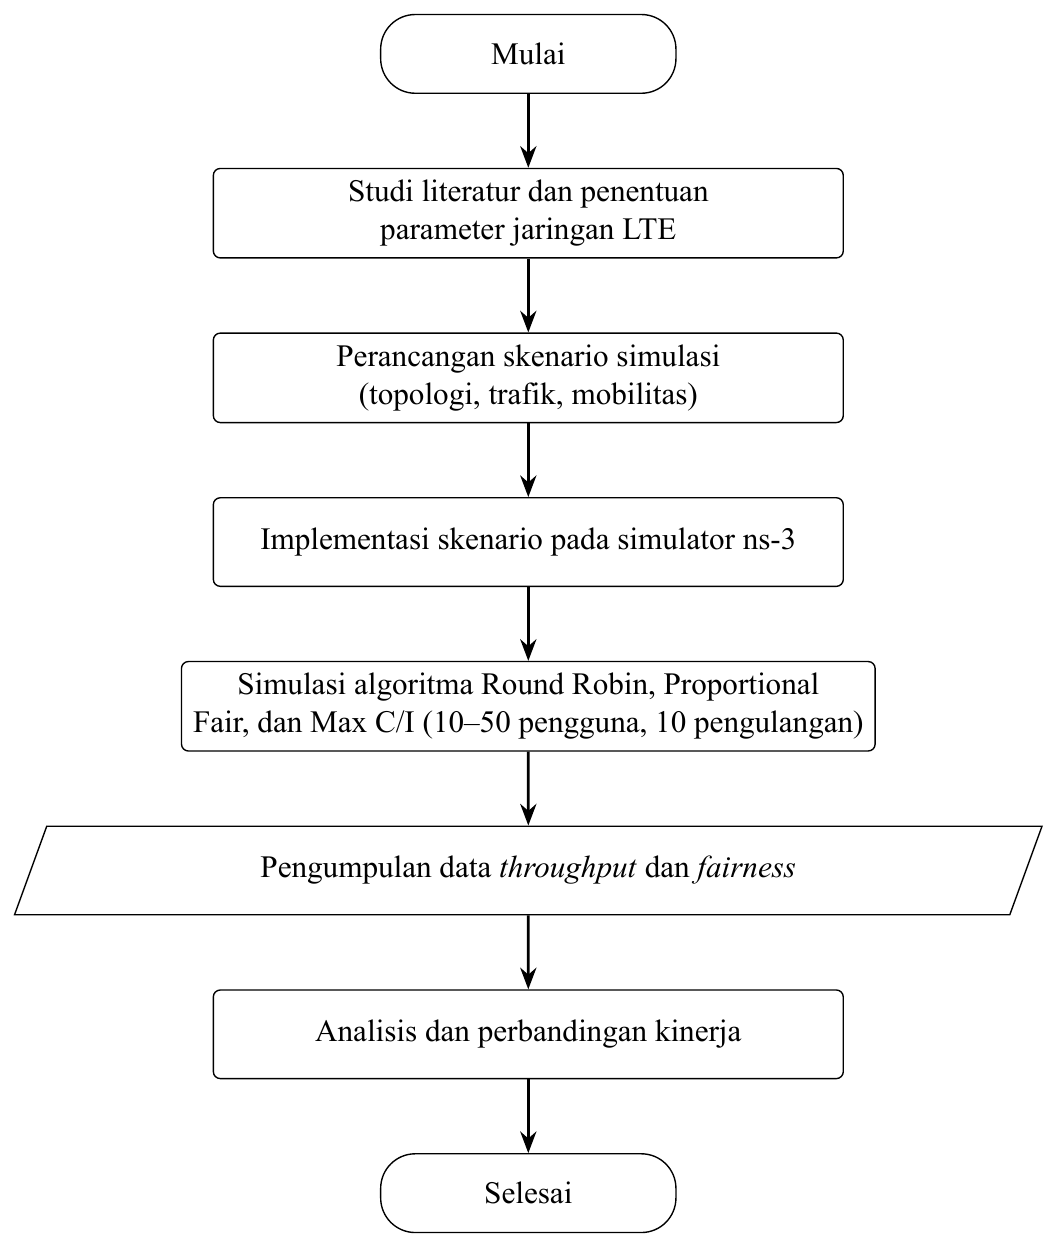
\includegraphics[width=0.52\textwidth]{../gambar/alur-penelitian.png}
\caption{Diagram alir tahapan penelitian}
\end{figure}

\section{Perancangan Skenario Simulasi}
Skenario simulasi terdiri atas satu eNodeB di pusat sel dengan radius 500 m dan sejumlah pengguna (UE) yang tersebar acak dan bergerak seperti pada Gambar 3.2. Parameter simulasi akan digunakan sesuai Tabel 3.1.

\begin{figure}[H]
\centering
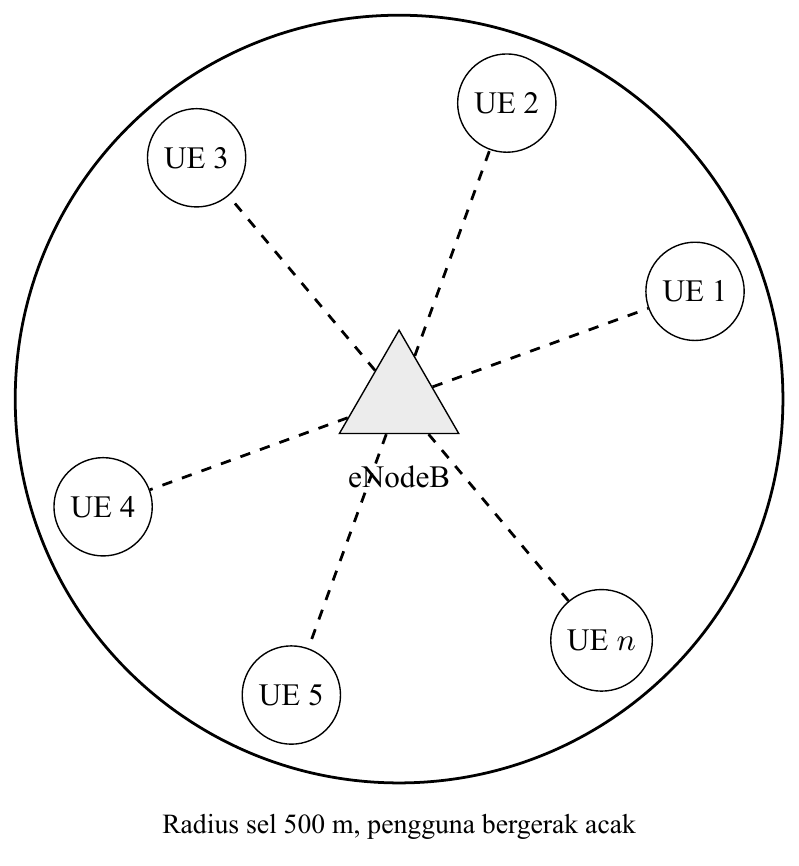
\includegraphics[width=0.45\textwidth]{../gambar/topologi.png}
\caption{Topologi simulasi satu sel LTE}
\end{figure}

\begin{singlespace}
\begin{longtable}{|p{0.42\linewidth}|p{0.46\linewidth}|}
\caption{Parameter simulasi}\\
\hline
\textbf{Parameter} & \textbf{Nilai} \\
\hline
Lebar pita \textit{downlink} & 20 MHz (100 RB) \\
\hline
Jumlah eNodeB & 1 \\
\hline
Radius sel & 500 m \\
\hline
Jumlah pengguna (UE) & 10, 20, 30, 40, 50 \\
\hline
Model mobilitas & \textit{Random walk}, kecepatan 3 km/jam \\
\hline
Model propagasi & Friis \\
\hline
Trafik & UDP \textit{downlink}, paket 1.024 byte, 1 Mbps per UE \\
\hline
Algoritma penjadwalan & RR, PF, Max C/I \\
\hline
Durasi simulasi & 60 detik \\
\hline
Pengulangan & 10 kali dengan \textit{seed} berbeda \\
\hline
\end{longtable}
\end{singlespace}

\section{Variabel dan Analisis Data}
Variabel bebas penelitian adalah algoritma penjadwalan (RR, PF, Max C/I) dan jumlah pengguna (10--50). Variabel terikatnya adalah \textit{throughput} total (Mbps) dan indeks \textit{fairness} Jain. Setiap kombinasi algoritma dan jumlah pengguna disimulasikan 10 kali dengan \textit{seed} acak berbeda, kemudian dihitung nilai rata-ratanya. Perbandingan antaralgoritma dinyatakan dalam persentase selisih terhadap algoritma RR sebagai acuan, dan disajikan dalam tabel dan grafik.

\needspace{10cm}
\section{Jadwal Pelaksanaan}
Penelitian direncanakan berlangsung selama enam bulan sebagaimana disajikan pada Tabel 3.2.

\begin{table}[H]
\caption{Jadwal pelaksanaan penelitian}
\centering
\begin{singlespace}
\renewcommand{\arraystretch}{1.8}
\setlength{\tabcolsep}{9pt}
\begin{tabular}{|c|p{4.8cm}|*{6}{c|}}
\hline
\multirow{2}{*}{\textbf{No}} & \multirow{2}{*}{\textbf{Kegiatan}} & \multicolumn{6}{c|}{\textbf{Bulan ke-}} \\
\cline{3-8}
 & & 1 & 2 & 3 & 4 & 5 & 6 \\
\hline
1 & Studi literatur & \isi & \isi & & & & \\
\hline
2 & Perancangan skenario simulasi & & \isi & \isi & & & \\
\hline
3 & Implementasi pada ns-3 & & & \isi & \isi & & \\
\hline
4 & Simulasi dan pengumpulan data & & & & \isi & \isi & \\
\hline
5 & Analisis data & & & & & \isi & \isi \\
\hline
6 & Penyusunan laporan dan seminar & & & & & & \isi \\
\hline
\end{tabular}
\end{singlespace}
\end{table}

% Daftar Pustaka (gaya APA edisi ke-7)
\babtp{DAFTAR PUSTAKA}
\begin{pustaka}
AlQahtani, S. A., \& Alhassany, M. (2013). Comparing different LTE scheduling schemes. \textit{2013 9th International Wireless Communications and Mobile Computing Conference (IWCMC)}, 264--269.

Andrews, M. (2007). A survey of scheduling theory in wireless data networks. \textit{Wireless Communications, 143}, 1--17.

Capozzi, F., Piro, G., Grieco, L. A., Boggia, G., \& Camarda, P. (2013). Downlink packet scheduling in LTE cellular networks: Key design issues and a survey. \textit{IEEE Communications Surveys \& Tutorials, 15}(2), 678--700.

Dahlman, E., Parkvall, S., \& Sk\"{o}ld, J. (2011). \textit{4G: LTE/LTE-Advanced for mobile broadband}. Academic Press.

Ghosh, A., Zhang, J., Andrews, J. G., \& Muhamed, R. (2010). \textit{Fundamentals of LTE}. Prentice Hall.

Jain, R. K. (1991). \textit{The art of computer systems performance analysis: Techniques for experimental design, measurement, simulation, and modeling}. John Wiley \& Sons.

ns-3 Consortium. (t.t.). \textit{ns-3 network simulator}. Diakses pada 21 Oktober 2026, dari \url{https://www.nsnam.org}

Xu, Y., \& Fischione, C. (2012). Real-time scheduling in LTE for smart grids. \textit{Proceedings of the 5th International Symposium on Communications, Control and Signal Processing}, 2--4.
\end{pustaka}


\end{document}
